\chapter{Mercury}
\label{sec:mercury}
Mercury \cite{mochi-core, mercury} is an asynchronous RPC framework purposefully built to efficiently provide communication services to HPC systems with high-performance fabrics. It provides an abstracted network implementation to enable transparent support to future systems and protocols, efficient use of existing native transport mechanisms, and support of large data arguments via the RDMA enabled interface. Moreover, it provides an asynchronous RPC interface, based on a callback system, that allows transfer of parameters and procedure calls in the context of both local and remote execution in order to completely remove the differentiation of communications between on and off-node.

The library allows the execution of arbitrary functions via a system of function tagging and callbacks, coupled to a queue system that saves procedure calls which are pending and still not executed. The receiving process drives the progress loop in which arguments are retrieved, function calls are executed, and the results are sent back to the origin node.

Additionally, the library offers the possibility of being ported to various systems since the network layer is abstracted and the application interface is based on a simple set of network primitives for both point-to-point messaging and one-sided RDMA. The network abstraction layer functionalities are implemented on top of different plugins. The plugin system can be considered as a \textit{compatibility} layer, which implements the communication functionalities offered by different protocols. Examples of plugins are Libfabric \cite{libfabric, ofi_plugin}, MPI \cite{mpi_plugin} and UCX \cite{openucx}, and multiple protocols are offered by each of the plugin, ranging from vendor-specific protocols to more classic ones like TCP and UDP.\newline

\section{RPC: a Mercury's perspective}
General RPC frameworks provide the possibility to serialize function parameters and ship them to a remote node that will execute the respective function call. As stated in \cite{mercury}, Mercury tries to address two main problems:
\begin{itemize}
    \item inability to take advantage of HPC high performance communication protocols: standard frameworks are usually designed on top of TCP/IP protocols, which represent a limitation over the performances often required by HPC systems;
    \item inability to transfer large amount of data: standard RPC frameworks doesn't allow (or discourage) transfer of large amount of data through the implemented mechanisms.
\end{itemize}

Mercury addresses these limitations by offering an asynchronous and flexible RPC interface specifically tailored for HPC systems. To do this, Mercury exposes an abstracted API to perform asynchronous RPC as well as large data transfer, and completely relies on the underlying network implementation provided by the plugins, in order to be independent from the used transport mechanism. As stated in \cite{mercury}, Mercury's main purpose is to serve as a basis for higher-level frameworks that need to remotely exchange data in a distributed environment, by offering a flexible interface completely decoupled from the underlying protocol and system specifications.

\section{Architecture}
Mercury is built on a two-layer architecture, as shown in \hr{fig:mercury-rpc-components}{Figure}, where each layer provides an abstraction for specific functionalities. The lowermost layer offers abstractions needed to provide networking functionalities such as point-to-point messaging, address lookup, remote memory access, progress and cancellation. The uppermost layer is further divided in two service-level components, referred to as \textit{RPC interface} and \textit{bulk data interface}. The RPC interface allows the programmer to remotely execute function calls, shipping function arguments and receiving results from the remote node; the bulk interface, instead, complements the RPC interface and allows large data transfer via the creation of memory descriptors, which enables the possibility to initiate raw memory transfers using remote memory access, whenever the underlying system provides it.\newline
\begin{figure}[H]
    \centering
    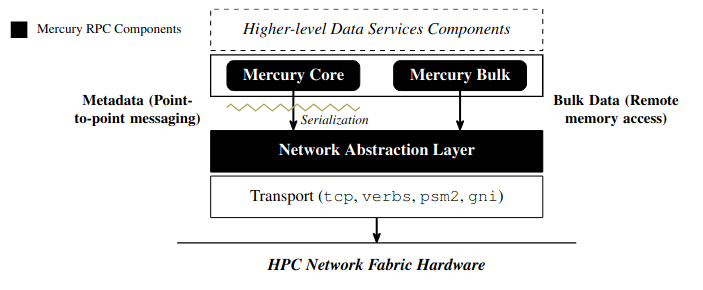
\includegraphics[width=0.8\linewidth]{res/RPC_components.png}
    \caption{Mercury RPC components in the software stack.}
    \label{fig:mercury-rpc-components}
\end{figure}

Mercury extends the functionalities of another project, called \textit{I/O Forwarding Scalability Layer} (IOFSL)\cite{iofsl}, which allows RPC calls specifically related to file-system-specific I/O operations. By extending this layer, Mercury allows to generate RPC calls to generic functions that can be dynamically defined and registered in the application using Mercury.

\subsection{Plugins}
\label{plugins}
The plugin functionalities are referred to as a ``\textit{support for various network protocols that can be easily added and selected at runtime}'' \cite{nal_guide}.
Given that Mercury's main aim is to leverage the high performance solutions provided by HPC network fabrics, which requires specific low-level vendor APIs, Mercury relies on plugins as an intermediate layer for network functionalities. In order to overcome the burden of implementing the network abstraction layer directly on top of those APIs, Mercury relies over various plugins for the implementation of functionalities like RDMA and point-to-point messaging. A multitude of plugins are provided by the framework, however the vast majority of them is under testing or being deprecated, leaving as ``stable'' only the ones related to Libfabric, UCX and shared-memory \cite{sm_plugin} for local nodes communication. We show in \S\ref{limitations} the main limitations we have encountered during testing of these plugins.\newline

Switching between various plugins is very simple and can be done by specifying a predefined string containing the desired plugin paired with the needed protocol to use during communications. Each plugin defines its own format, but common fields are shared among the configuration strings of various plugins, and they mostly refer to the type of plugin and the protocol to be used. Format of strings is provided in \hr{tab:mercury-string}{Table}.

\begingroup
\renewcommand{\arraystretch}{1.3} % Default value: 1
\begin{table}[H]
\begin{center}
    \begin{tabular}{ | c | c | c |}
    %\begin{adjustwidth}{0cm}{}
         \hline
         \textbf{Plugin} & \textbf{Protocol} & \textbf{Initialization format}\\ [0.5ex] 
         \hline\hline
         ofi & tcp & \text{ofi+tcp[://\textlangle{}hostname,IP,interface name\textrangle{}:\textlangle{}port\textrangle{}]}\\
         & verbs & ofi+verbs[://[domain/]\textlangle{}hostname,IP,interface name\textrangle{}:\textlangle{}port\textrangle{}]\\
         & psm2 & ofi+psm2\\
         & gni & ofi+gni[://\textlangle{}hostname,IP,interface name\textrangle{}]\\\hline
         ucx & all & ucx+all[://[net\_device/]\textlangle{}hostname,IP,interface name\textrangle{}:\textlangle{}port\textrangle{}]\\
         & tcp & ucx+tcp[://[net\_device/]\textlangle{}hostname,IP,interface name\textrangle{}:\textlangle{}port\textrangle{}]\\
         & rc,ud & ucx+\textlangle{}rc,ud\textrangle{}[://[net\_device/]\textlangle{}hostname,IP,interface name\textrangle{}:\textlangle{}port\textrangle{}]\\\hline
         na & sm & na+sm[://\textlangle{}shm\_prefix\textrangle{}]\\\hline
         mpi & dynamic, static & mpi+\textlangle{}dynamic, static\textrangle{}\\\hline
    \end{tabular}
    \caption{Mercury plugin's initialization format.}
    \label{tab:mercury-string}
    %\end{adjustwidth}
    \end{center}
\end{table}
\endgroup

Note, however, that plugins may behave differently regarding how the format string is provided, in fact plugins do not manage incomplete or incorrect configuration strings uniformly. Some of these issues are reported in \S\ref{limitations}.

\subsection{Network Abstraction Layer}
\label{sec:NAL}
The Network Abstraction Layer (NAL) provides an abstraction of the network infrastructure above which the communications are executed. It is a simple abstraction which only provides limited functionalities, like address lookup, point-to-point messaging, remote memory access, progress, and cancellation.\newline

The abstractions provided by this layer allows the uppermost layers to be completely agnostic of the underlying communication protocol implemented via the plugin system. Moreover, The API is non-blocking and uses a callback mechanism to provide asynchronous execution. Progress is driven by API calls which allows user callbacks to be placed in completion queue and retrieved for execution.\newline

Mercury refers to communicating nodes as \ttt{origin} and \ttt{target}, indicating respectively the node issuing the request and the node receiving it. Both origin and target nodes must specify the desired plugin/protocol pair at initialization phase, by providing a string as described in \S\ref{plugins}. Since a node can both provide and ask for services, the only time a server-specific behaviour is defined only refers to initialization, where the user can specify if the current node will be listening for incoming RPCs. Besides this, no more server/client concepts are used in the following.\newline

The functionalities offered by the NAL refers to three main mechanisms:
\begin{itemize}
    \item expected messages: requires a \textit{receive} operation to be pre-posted by the target. Therefore, this requires the origin node to be known in advance, before the receive operation is posted. If the receive operation is not posted before the message is sent, it can be dropped;
    \item unexpected messages: does not require the target to post a receive operation for the message, and they can arrive from any source. The target can retrieve received messages in an asynchronous way. These messages are allowed to be dropped, but the plugin can decide to queue them anyway;
    \item remote memory access: allows registration of memory chunks which can be later accessed by target nodes. Abstractions are provided through API which contains operations generally provided by most RDMA protocols.
\end{itemize}

The network abstraction is designed to allow emulation of one-sided operations, such as RDMA, on top of two-sided operations. In this way, Mercury can easily adapt to protocols which only supports fixed operations, like TCP/IP ones, where one-sided communications are not possible.


\subsection{RPC Layer}
The RPC layer allows nodes to issue remote calls, and it is based on the messaging model described in \S\ref{sec:NAL}. RPC requests are based on the common knowledge of origin and target nodes on how to encode and decode function parameters and return values.\newline
\begin{figure}[H]
    \centering
    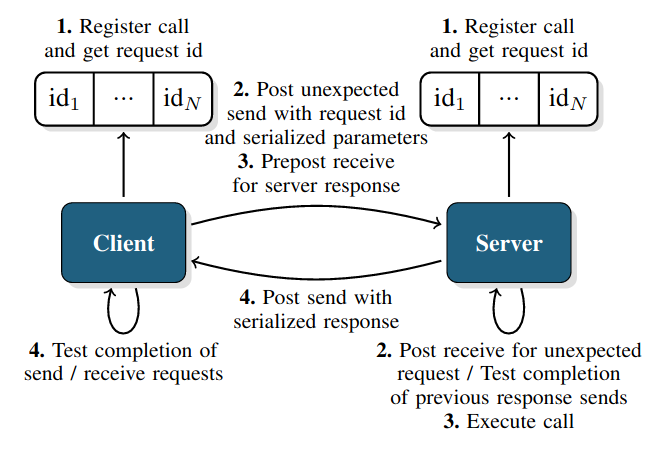
\includegraphics[width=0.6\linewidth]{res/rpc-flow.png}
    \caption{Execution flow of RPC call. }
    \label{fig:rpc-flow}
\end{figure}

Mercury provides mechanisms to support a set of generic function calls avoiding hard-coded routines. To allow this, origin and target nodes must register a unique function name along with encoding and decoding routines by using shared input/output types. We postpone the precise description of the registration process to \S\ref{sec:rpc-reg}, since Margo introduces few additional steps, which are the ones that are actually used to implement FastFlow's communication classes. We show in \hr{fig:rpc-flow}{Figure} a usual flow of execution needed by both origin and target nodes to execute a RPC request. The registered function is mapped to an ID which will be used in all the communications between the two nodes. A further step is needed by the target, which must register a callback that will be executed every time that ID is received. Once the functions are registered, the origin sends an \textit{unexpected} message to the target.\newline

Two situation may occur during an RPC request, and different mechanisms are used to guarantee full asynchrony:
\begin{itemize}
    \item the RPC call expects a response from the target: the origin node prepares its memory buffer to receive the response and uses the buffer to pre-posts an \textit{expected receive}. At the reception of the response, the origin node can retrieve the response from the callback queue and proceed;
    \item the RPC call does not expect a response from the target: the origin node, at the moment of RPC registration, declares that this RPC does not expect a response. An RPC of this kind allows the origin node to proceed without posting a receive operation, progress can be made as soon as the request is sent to the target.
\end{itemize}

From the target side, receiving an \textit{unexpected} message with a specified ID translates in the execution of the callback registered at startup by decoding the parameters sent by the origin, and sending the outputs by encoding them at the end of execution, if the registered RPC expects a response.
\subsection{Bulk Layer}
This layer allows to send large data by avoiding intermediate memory copies. It is performed by creating a local memory handle which points to previously registered areas of memory (not necessarily contiguous) which the target node can access via RDMA operations. The bulk layer is directly built on top of the RDMA interface defined in the network abstraction layer. \newline

\begin{figure}[H]
    \centering
    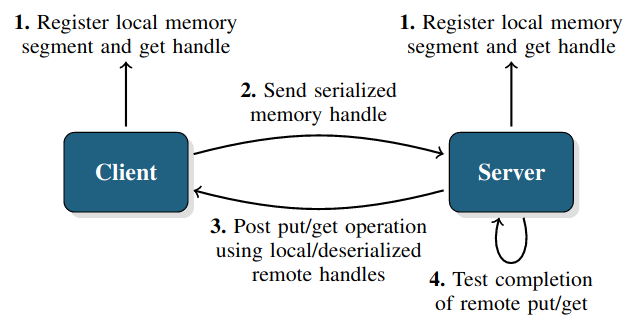
\includegraphics[width=0.6\linewidth]{res/bulk-flow.png}
    \caption{Execution flow of bulk request.}
    \label{fig:bulk-flow}
\end{figure}

A typical execution flow for a bulk request is depicted in \hr{fig:bulk-flow}{Figure}. The target node manages all the bulk transfers in order to be able to control the data flow and protect its memory from concurrent accesses. This operation is one-sided, and it is started by the origin node which creates a bulk data descriptor, serializes it, and send the serialized descriptor to the target as an argument via a specific RPC request. Once the descriptor has been deserialized by the target, two situations can occur. The request can be related to \textit{consumption} or \textit{production of data}. In both cases the target node creates a memory handle to manage the request, allocating the necessary memory. However, in the first case the target initiates a remote \texttt{read} operation before performing the function call, in the second case the target executes the call and initiates a remote \texttt{write} operation with the produced results.\newline

Memory handles are an important building block for memory transfer, in particular in such cases where non-contiguous memory is to be transferred. The memory of the communicating nodes is abstracted by the memory handle and allows to access memory in a transparent way without modifications to the process described above.

\section{Resilience and Fault Tolerance}
The fault tolerance mechanism is mainly provided by the possibility to interrupt calls and reclaim resources of pending operations after these have been signaled as \textit{cancelled}. Cancellation is an asynchronous and local operation. From a user perspective, completion of offloaded operations is known only when the associated callback is placed in the local queue of pending operations. When a callback is triggered and the operation was locally canceled by the user, that operation is reported as canceled and aborted.\newline

A basic flow of events related to the cancellation of an operation is shown in \hyperref[fig:op-cancel]{\textbf{Figure \ref{fig:op-cancel}}}.

\begin{figure}[H]
    \centering
    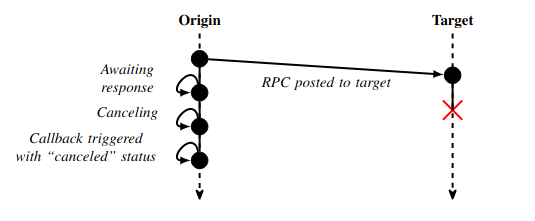
\includegraphics[width=0.6\linewidth]{res/op-cancel.png}
    \caption{Cancellation of an RPC operation.}
    \label{fig:op-cancel}
\end{figure}

\section{Dependencies}
As reported by \cite{merc_git}, the dependencies are mostly related to the intended plugin to integrate inside a specific application. No further requirements are specified by the Mercury's developers as needed for the installation and use of their framework.


\section{Mercury analysis}
\label{sec:mercury-analysis}
Mercury comes with lots of functionalities and drawbacks. We list in this section all the advantages and the main limitations of the Mercury framework encountered during the testing phase, which are therefore shared by all the higher-level libraries which are based on it.

\subsection{Advantages}
Mercury's interface allows to easily enable communication using a system of plugin which offers compatibility with a multitude of network and vendor specific protocols. The Mercury library, once again, shows the importance of having an abstraction layer to provide efficient use of underlying protocols without having a complete expertise on how they work. Being able to address different needs and to leverage the functionalities of different systems, by the means of a general API, makes implementing communication on such systems painless and less error prone. Moreover, Mercury's capability of handling different protocols with no code changes at all allows portability of applications to new systems which may provide only vendor specific protocols or which does not offer support to common transports such as TCP or MPI.

\subsection{Limitations}
\label{limitations}
Mercury, however, is not exempt from problems and limitations. In this section we gathered all the main limitations that are known and which we discovered during the testing phase of the presented framework. As specified in \S\ref{plugins}, MPI plugin is deprecated and not maintained \cite{git_mercury_mpi}. In fact, Mercury's developers suggest the use of libfabric plugin to leverage efficient HPC communication mechanisms, and UCX plugin as a general purpose plugin. As specified in \cite{nal_guide}, MPI is considered to be present in almost all systems, and the functionality offered by the NAL are only intended for prototyping and testing, this suggesting that in case an MPI implementation is needed, one shouldn't rely on Mercury's interface.\newline

Further limitations found during the testing of this library are mostly related to the limited support of the Libfabric plugin paired with TCP transport \cite{mercury_plugins}, which is intended to use for testing and debugging applications on machines that do not provide high performance fabric protocols \cite{ofi_tcp}. Problems about this specific transport were already reported \cite{ofi_tcp, git_mercury_tcp, git_mercury_tcp332}, and during testing the main that we noticed are:
\begin{itemize}
    \item During reply phase of RPC request using \texttt{ofi+tcp}, information about public IP of origin node are not used. This resulting in a lost packet in case the origin node was behind NAT, probably due to the \textit{emulated} source addressing, as stated in \cite{ofi_plugin}. The same does not happen by using \texttt{ofi+sockets}, which use is discouraged as per \cite{mercury_plugins};
    \item Various problems related to termination of nodes which issued a request that couldn't be fulfilled, as also reported in \cite{git_mercury_tcp};
    \item As per \cite{libfabric-github}, the sockets provider has been deprecated in favor of the tcp one. 
\end{itemize}

Other plugins, such as UCX \cite{ucx_plugin}, showed some problem in connecting nodes situated in different networks, mostly due to the fact that the plugin provided by Mercury struggles to bind the socket address to the specified one. However, it is able to establish a connection between endpoints situated in the same subnetwork.\newline

Given the requirements for the FastFlow distributed version, the internal limitations of the Mercury framework could be too tight to allow its extensive utilization as a final communication library. However, the provided plugins and functionalities could anyway serve as a prototyping library in order to develop FastFlow communication layer APIs, in order to painlessly switch to a different communication framework in the future.\newline

In fact, as we show in \S\ref{sec:margo}, the composition of the Mercury framework with higher-level abstractions allows to easily develop communication nodes to handle multiple endpoints at once without struggling with the explicit progress mechanism provided by Mercury. For this reason, in the next sections we introduce the libraries used by the higher-level abstractions which use Mercury framework as a core building block to provide RPC functionalities in an automatized way.

We show, for each of the analyzed libraries and frameworks, which are their advantages and drawbacks, with special focus on lowering the amount of dependencies and minimizing the knowledge of the communication layer about the data that are exchanged between nodes, in order to create communicating nodes completely agnostic about the types used during computation, allowing also for parallelization of the serialization process and reducing the computation needed at the ``edge'' of each group.\newline

Besides the limitations we have analyzed, which are mostly related to technical aspects and not on the usability of the presented frameworks, the simplicity of creating communication nodes and connecting them via a high-level communication library such as Margo, without requiring too many modification in the original application code, can be a good driver to experiment and develop an initial set of API calls which will allow to extend the communication layer functionalities and plug in a broader set of protocols which are still not supported by the used frameworks. Having an independent API is a natural and important step to remove strict dependencies from each of the technologies used to implement the communication functionalities, allowing extensibility with little to no changes in existing code.
Besides the limitations we have found during the experimentation with the analyzed libraries, our analysis on those frameworks was anyway important to understand the power and utility of having a high level abstraction on top of very specific APIs which requires a deep understanding of how the underlying infrastructure works. Hence, it is conceptually interesting and it could be very helpful in the implementation of the final communication layer to retain some of the concepts introduced by the \textit{Mochi core} building blocks.
